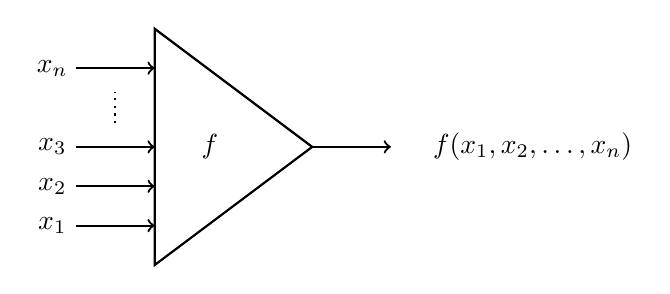
\begin{tikzpicture}
    % Draw the triangle with vertical left edge
    \draw[thick, fill=white] (0,0) -- (0,3) -- (2,1.5) -- cycle;

    % Draw input arrows
    \draw[->, thick] (-1,0.5) -- (0,0.5);
    \draw[->, thick] (-1,1) -- (0,1);
    \draw[->, thick] (-1,1.5) -- (0,1.5);
    \draw[dotted, thick] (-0.5,1.8) -- (-0.5,2.2);
    \draw[->, thick] (-1,2.5) -- (0,2.5);

    % Draw output arrow
    \draw[->, thick] (2,1.5) -- (3,1.5);

    % Add labels
    \node at (0.7,1.5) {$f$};
    \node at (-1.3,0.5) {$x_1$};
    \node at (-1.3,1) {$x_2$};
    \node at (-1.3,1.5) {$x_3$};
    \node at (4.8,1.5) {$f(x_1,x_2,\ldots,x_n)$};
    \node at (-1.3,2.5) {$x_n$};
\end{tikzpicture}